\documentclass[12pt]{article}
\usepackage{amsmath}
\usepackage[top=1in, bottom=1in, left=0.8in, right=1in]{geometry}
\usepackage{multicol}
\usepackage{wrapfig}
\usepackage{listings}
\usepackage{enumitem}
\usepackage{comment}
\usepackage{tikz}
\usepackage{hyperref}
\usepackage{caption}
\usepackage{subcaption}
\usepackage[ruled,vlined]{algorithm2e}
\lstset{language=Java, basicstyle={\small\ttfamily}, columns=flexible, belowskip=0mm}
\setlength{\columnsep}{0.1pc}

\begin{document}

\noindent
CS 440: Intro to Artificial Intelligence \hfill Assignment 2A\newline
Fall 2022 \hfill Due November 23, 2022, 11:59 p.m.

\noindent
\rule{\linewidth}{0.4pt}

\vspace{.5cm}

\textbf{Names}: Will Chen, Noel Declaro, Afsana Rahman

\vspace{.5cm}

\textbf{Overview}:  This document contains answers to Problems 1-4 in Assignment 2. 

\noindent
\rule{\linewidth}{0.4pt}

\vspace{.5cm}

%%%%%%%%%%%%%%%%%%%%%%%%%%%%%%%%
\textbf{Question 1 (10 points):} Consider the following Bayesian network, where variables $A$ through $E$ are all boolean valued:

\begin{figure}[h]
    \centering
    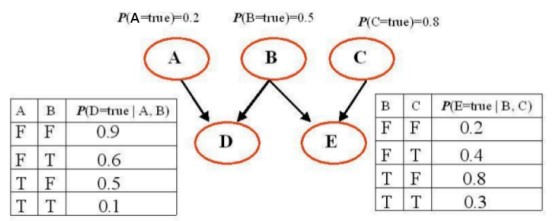
\includegraphics{images/probdescrips/prob1.jpg}
	\caption{}
	\label{fig:prob1}
\end{figure}

For the sake of shorthand, assume for any random variable $A,B,C,D,E$ in this network, its corresponding lowercase letter refers to its true value being $true$ and its negation being $false$ (e.g., $a \iff A = true, \neg a \iff A = false$).

\begin{enumerate}[label=(\alph*)]
    \item \textbf{Probability of all true.} We want to find $P(a,b,c,d,e)$.
        \begin{itemize}
            \item $P(a) = 0.2$
            \item $P(b) = 0.5$
            \item $P(c) = 0.8$
            \item $P(d | a, b) = 0.1$
            \item $P(e | b, c) = 0.3$
        \end{itemize}

        $P(a,b,c,d,e) = P(a) \times P(b) \times P(c) \times P(d|a,b) \times P(e|b,c) \\$
        $= 0.2 \times 0.5 \times 0.8 \times 0.1 \times 0.3 \\$ 
        $= 0.0024$
    
    \item \textbf{Probability of all false.} We want to find $P(\neg a, \neg b, \neg c, \neg d, \neg e)$.
        \begin{itemize}
            \item $P(\neg a) = 0.8$
            \item $P(\neg b) = 0.5$
            \item $P(\neg c) = 0.2$
            \item $P(\neg d | \neg a, \neg b) = 0.1$
            \item $P(\neg e | \neg b, \neg c) = 0.3$
        \end{itemize}
        $P(\neg a, \neg b, \neg c\, \neg d, \neg e) = P(\neg a) \times P(\neg b) \times P(\neg c) \times P(\neg d|\neg a, \neg b) \times P(\neg e|\neg b, \neg c) \\$
        $= 0.8 \times 0.5 \times 0.2 \times 0.9 \times 0.2 \\$ 
        $= 0.0064$

    \item \textbf{Probability A is false given rest are true.}
        \begin{itemize}
            \item $P(\neg a) = 0.8$
            \item $P(b) = 0.5$
            \item $P(c) = 0.8$
            \item $P(d | \neg a, b) = 0.6$
            \item $P(e | b, c) = 0.3$
        \end{itemize}
         $P(\neg a,b,c,d,e) = P(\neg a) \times P(b) \times P(c) \times P(d|\neg a,b) \times P(e|b,c) \\$
        $= 0.8 \times 0.5 \times 0.8 \times 0.6 \times 0.3 \\$ 
        $= 0.0576$
\end{enumerate}

\rule{\linewidth}{0.4pt}
\vspace{.2cm}

%%%%%%%%%%%%%%%%%%%%%%%%%%%%%%%%
\textbf{Question 2 (10 points):}

\begin{figure}[h]
    \centering
    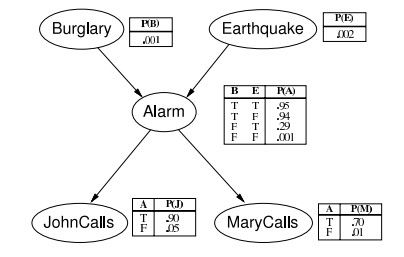
\includegraphics{images/probdescrips/prob2.jpg}
	\caption{}
	\label{fig:prob2}
\end{figure}

\begin{enumerate}[label=(\alph*)]
    \item \textbf{Variable elimination.} Given the query $P(Burglary | JohnCalls = true, MaryCalls = true)$, we can rewrite as:
    \begin{equation}
        P(B | j, m) = \alpha P(B) \sum_e P(e) \sum_a P(a | B,e)P(j|a)P(m|a)
    \end{equation} 
    We can then begin to eliminate variables, starting with the variables including $a$: 
    
    \begin{center}
        $ P(B | j,m) = \alpha P(B) \sum_e P(e)
        \begin{pmatrix}
             0.598582 & 0.18655\\
             0.59223 & 0.0011295
        \end{pmatrix}$
    \end{center}
        
    And then "eliminate" $\sum_e P(e)$:
    \begin{center}
        $ P(B | j,m) = \alpha P(B) 
        \begin{pmatrix}
             0.0002 * 0.598525 + 0.998 * 0.59223\\
             0.0002 * 0.183055 + 0.998 * 0.0011295
        \end{pmatrix}$
    \end{center}
    
    And then "eliminate" $P(B)$:

    \begin{center}
        $P(B | j,m) = \alpha
        \begin{pmatrix}
             0.001 * 0.59224259 \\
             0.999 * 0.001491858
        \end{pmatrix} $
    \end{center}

    And then normalize. So we have $P(B | j,m) = <0.284, 0.716>$.
    
    \item \textbf{Number of operations.}
        \begin{itemize}
            \item \textbf{Variable elimination.} In this problem, computing takes two sets of 3 operations. Since there are 11 total operations in burglary, we get 2*11 + 3 = 25 operations.
            \item \textbf{Enumeration.} (As taken from the lecture slides) The expression is computed by adding four terms, each computed by multiplying five numbers. So there is a total of 40 operations (since time is doubled due to computation of $\alpha$).
        \end{itemize}
        
    \item \textbf{Chain Bayesian network.} 
        \begin{itemize}
            \item \textbf{Variable elimination.} There are $n-2$ variables to sum over with $n-1$ multiplications each.
            
            $\\ P(X_1 | X_n = true) = \alpha \sum_{X_2 ... X_{n-1}} P(X_n = true | X_{n-1})P(X_{n-1} | X_{n-2}) ... P(X_2 | X_1)P(X_1)\\$
            
            $ P(X_1 | X_n = true) = \alpha \sum_{X_{n-1}} P(X_n = true | X_{n-1}) \sum_{X_{n-2}} P(X_{n-1} | X_{n-2}) ... \sum_{X_2}P(X_3 | X_2)\\$
            
            There are $n-2$ summations on each; it has running time $O(n)$.
            \item \textbf{Enumeration.} Two binary search trees can be used for each value of $x_1$ with depths $n-2$, giving total work done to be $O(2n)$.
        \end{itemize}
    
\end{enumerate}

\vspace{0.4cm}

%%%%%%%%%%%%%%%%%%%%%%%%%%%%%%%%
\textbf{Question 3 (15 points):} Please note the code used in this question was included in the zip file of our submission.

\begin{figure}[h]
    \centering
    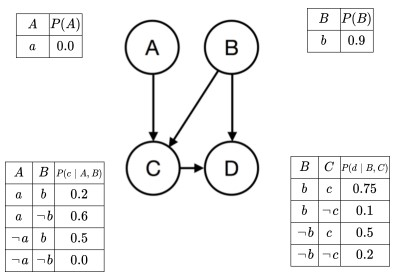
\includegraphics{images/probdescrips/prob3.jpg}
	\caption{}
	\label{fig:prob3}
\end{figure}

\begin{enumerate}[label=(\alph*)]
    \item \textbf{Enumeration.}
        \begin{itemize}
            \item $P(d|c)$. To find this probability, we'll introduce $\alpha$ and sum over $a$ and $b$.
            $\\ P(d|c) = \alpha P(d,c) = \alpha P(a,b,c,d)\\$
            $= \alpha \sum_a \sum_b P(a) P(b) P(c|a,b) P(d|b,c)\\$
            $= \alpha \sum_a P(a) \sum_b P(b) P(c|a,b) P(d|b,c)\\$
            $= \alpha <0.3375, 0.1125> = <0.75, 0.25>\\$
            This means $P(d|c)$ = 0.75.
            \item $P(b|c)$. To find this probability, we'll introduce $\alpha$ and sum over $a$ and $d$.
            $\\ P(b|c) = \alpha P(b,c) = \alpha P(a,b,c,d)\\$
            $= \alpha \sum_a \sum_d P(a) P(b) P(c|a,b) P(d|b,c)\\$
            $= \alpha P(b) \sum_a P(a) P(c|a,b) \sum_d  P(d|b,c)\\$
            $= \alpha <0.45, 0> = <1, 0>\\$
            This means $P(b|c)$ = 1.
            \item $P(d|\neg a,b)$. To find this probability, we'll introduce $\alpha$ and sum over $c$.
            $\\ P(d|\neg a, b) = \alpha P(d,a,b) = \alpha P(a,b,c,d)\\$
            $= \alpha \sum_c P(a) P(b) P(c|a,b) P(d|b,c)\\$
            $= \alpha P(a) P(b) \sum_a P(c|a,b) \sum_d  P(d|b,c)\\$
            $= \alpha <0.3825, 0.5157> = <0.425, 0.575>\\$
            This means $P(d|\neg a, b)$ = 0.425.
        \end{itemize}
    \item \textbf{Likelihood and rejection sampling.} The results of 1000 samples are shown in Figure 4. The approximation using rejection sampling was fairly accurate to the true probabilities. The approximation using likelihood was similar.
    \begin{figure}
          \begin{subfigure}{0.5\textwidth}
            \centering
            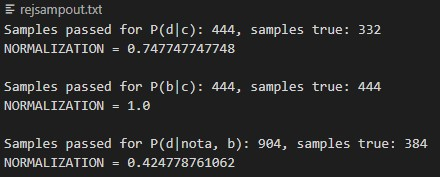
\includegraphics[width=\textwidth]{images/prob3/txtresults/3b.jpg}
            \caption{}
            \label{fig:fig3a}
          \end{subfigure}
          \begin{subfigure}{0.5\textwidth}
            \centering
            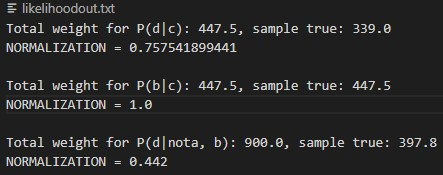
\includegraphics[width=\textwidth]{images/prob3/txtresults/3b1.jpg}
            \caption{}
            \label{fig:fig3b}
          \end{subfigure}
          \caption{Results of rejection sampling and likelihood weighting, respectively, for 1000 samples.}
      \end{figure}
      
    \item \textbf{Number of samples.} The plot of probability versus number of samples is shown in Figure 5. The number of samples was changed manually in the code from the previous part. The graphs were also created manually. The likelihood weighting was shown to converge much faster than the rejection sampling.

    \begin{figure}
          \begin{subfigure}{0.5\textwidth}
            \centering
            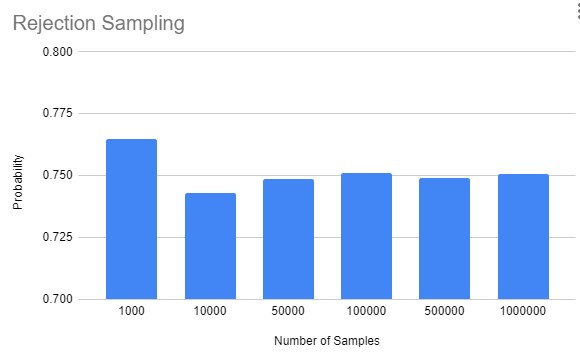
\includegraphics[width=\textwidth]{images/prob3/graphresults/3ba.jpg}
            \caption{}
            \label{fig:fig3a}
          \end{subfigure}
          \begin{subfigure}{0.5\textwidth}
            \centering
            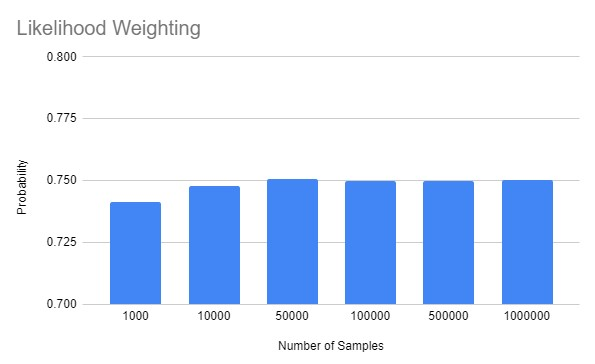
\includegraphics[width=\textwidth]{images/prob3/graphresults/3bb.jpg}
            \caption{}
            \label{fig:fig3b}
          \end{subfigure}
          \caption{Plots of rejection sampling and likelihood weighting, respectively, for increasing samples.}
    \end{figure}
    
\end{enumerate}

\rule{\linewidth}{0.4pt}
\vspace{.2cm}

%%%%%%%%%%%%%%%%%%%%%%%%%%%%%%%%
\textbf{Question 4 (15 points):}

\begin{figure}[h]
    \centering
    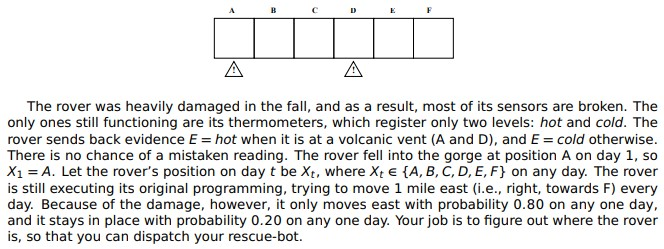
\includegraphics{images/probdescrips/prob4.jpg}
	\caption{}
	\label{fig:prob4}
\end{figure}

\begin{enumerate}[label=(\alph*)]
    \item \textbf{Filtering.} We want to find the probability distribution over the rover's position on day 3, given the observations $(E_1 = hot, E_2 = cold, E_3 = cold)$. It is important to note that the rover does not misread temperature, and only moves 1 mile east per day or stays in place for the day. 
    
    This means that the minimum distance the rover could move is 0 miles, meaning it stays in position A, and the maximum distance is 2 miles to position C (since there is no movement on day 1). This means that it is automatically impossible for the rover to be at positions D, E, or F, or in other words, the probability of the rover being positioned anywhere here on day 3 is 0.

    Now, since $E_2 = cold$, and we know the rover does not make false temperature reports, and the rover only moves east, the rover must be at position B on day 2 (making the probability of the rover being at position A on day 3 therefore 0). Since $E_3 = cold$ as well, there is a chance the rover could have either stayed in place, or moved to position C, meaning the probability distribution on day 3 for the rover would be:
    \begin{center}
        DAY 3: $A = 0, B = 0.2, C = 0.8, D = 0, E = 0, F = 0$
    \end{center}
    
    \item \textbf{Smoothing.} Like above, we want to find the probability distribution of the rover's position, except now on day 2. As explained above, since the rover does not make false temperature reports, and we have recorded $E_2 = cold$, then we know the rover position cannot be A or D. We also know that since the rover only moves east, 1 mile per day maximum, it cannot have gone past position C (non-inclusive) before day 3. Therefore, the rover must be at position B on day 2 given the evidence, i.e.,
    \begin{center}
        DAY 2: $A = 0, B = 1, C = 0, D = 0, E = 0, F = 0$
    \end{center}
    
    \item \textbf{Most Likely Explanation.} The possible sequences that may have occurred on the first three days are either:
        \begin{itemize}
            \item The rover starts at A, moves to B on day 2, and stay on B for day 3. OR
            \item The rover starts at A, moves to B on day 2, and moves to C on day 3.
        \end{itemize}
    The only difference between the two sequences is that the rover either moves from or stays at position B on day 3. Since the former is more likely (0.8 versus 0.2 chance), the more likely $overall$ sequence is the one where the rover keeps moving east, i.e., position sequence A, B, C for days 1,2,3, respectively.
    
    \item \textbf{Prediction.} Given the original sequence of temperature readings, $E_1 = hot, E_2 = cold, E_3 = cold$, we want to find the probability of the next sequence $E_4 = hot, E_5 = hot, E_6 = cold$. The only possible way for the readings to be accurately $E_3 = cold, E_4 = hot$ is for the rover to be at position C on day 3, and then move to position D on day 4. Similarly, the $only$ possibly way for the rover to read "hot" two days in a row is if it stays on D for two days. $Similarly$, the $only$ way for the rover to move from hot to cold is for the rover to be at position D and then move to E. In summary, the only possible location sequence for all the evidence to be true is (for days 1-6 in chronological order) A, B, C, D, D, E.

    As determined in part (a), the probability of the rover being at position C on day 3 is 0.8; the chance of moving east on day 4 is also 0.8; the chance of it staying at its new location (D) on day 5 is 0.2; and the chance of it moving east on day 6 is 0.8. Therefore, the probability of the new sequence occurring given the previous one is $0.8 * 0.8 * 0.2 * 0.8 = 0.1024$.
    
    \item \textbf{Prediction.} Basing off part (a)'s probability distribution:
    \begin{center}
        DAY 3: $A = 0, B = 0.2, C = 0.8, D = 0, E = 0, F = 0$
    \end{center}
    we can build predictions for the next day based the on the information we are given. Since temperature is not taken into account, we only need to regard the probabilities of the rover's movement.

    Regarding day 4, if we assume that the rover is at position B, there is a 0.2 chance it stays there, and 0.8 percent chance it moves east to position C. Since the probability of being at position B was already 0.2 on day 3, the chance of staying there would be $0.2 * 0.2 = 0.04$, and the probability of moving from there would be $0.2 * 0.8 = 0.16$. The same logic applies to position C: the chance of being at position C on day 3 is 0.8, there is 0.2 chance of staying there, and 0.8 chance of moving east to position D. Therefore, if assuming we start at position C, the probability of staying there is $0.8 * 0.2 = 0.16$ and the probability of moving to position D is $0.8 * 0.8 = 0.64$. In summary:
    \begin{center}
        DAY 4: $A = 0, B = 0.04, C = 0.16 + 0.16 = 0.32, D = 0.64, E = 0, F = 0$
    \end{center}
    which is normalized. We repeat this process for day 5: 
    \begin{itemize}
        \item \textbf{Position B.} There is a 0.04 chance of the rover being here on day 4, and 0.2 chance of it staying for day 5, so the rover has a $0.04 * 0.2 = 0.008$ chance overall of being there on day 5.
        \item \textbf{Position C.} There is a 0.04 chance of the rover being at position B on day 4 with 0.8 chance of moving to position C, meaning this course of action has $0.04 * 0.8 = 0.032$ chance of happening. There is also a 0.32 chance the rover is already there on day 4, and 0.2 chance it may stay there for day 5, meaning there is $0.32 * 0.2 = 0.064$ chance of this course of actions occurring. This means the overall chance of the rover being here on day 5 is $0.032 + 0.064 = 0.096$.
        \item \textbf{Position D.} There is a 0.32 chance of the rover being at position C on day 4 with 0.8 chance of moving to position D, meaning this course of action has $0.32 * 0.8 = 0.256$ chance of happening. There is also a 0.64 chance the rover is already there on day 4, and 0.2 chance it may stay there for day 5, meaning there is $0.64 * 0.2 = 0.128$ chance of this course of actions occurring. This means the overall chance of the rover being here on day 5 is $0.256 + 0.128 = 0.384$.
        \item \textbf{Position E.} This is the furthest possible position the rover can go, as it has not been explored yet. There is a 0.64 chance the rover is at position D at day 4, and 0.8 chance the rover will move here on day 5, so the rover has $0.64 * 0.8 = 0.512$ chance of being here on day 5.
    \end{itemize}
    With normalization of the values determined above:
    \begin{center}
        DAY 5: $A = 0, B = 0.008, C = 0.096, D = 0.384, E = 0.512, F = 0$
    \end{center}
\end{enumerate}


\end{document}
